\documentclass[11pt]{article}
\usepackage[T1]{fontenc}
\usepackage[margin=1.2in,top=0.6in,bottom=0.6in]{geometry}
\usepackage[bookmarks,colorlinks=true,linkcolor=blue,urlcolor=blue]{hyperref}
\usepackage{url}
\usepackage{tabularx}
\usepackage{graphicx}
\usepackage{placeins}
\usepackage{paralist}
\usepackage{makecell}
\usepackage{colortbl}
\usepackage{gensymb}
\usepackage{textcomp}
%\usepackage[osf]{libertine}
\usepackage{zi4}
\usepackage{float}
\usepackage[libertine,cmbraces]{newtxmath}

% table lines
\newcommand{\thinhline}{\Xhline{1\arrayrulewidth}}
\newcommand{\thickhline}{\Xhline{2.5\arrayrulewidth}}

\begin{document}

\title{AKL-PT1 2 GHz Passive Probe Operator Manual}
\author{Antikernel Labs}
\date{\today}

\maketitle
\begin{abstract} \normalsize
This document is the user manual for the Antikernel Labs AKL-PT1 2 GHz passive transmission line probe.
\end{abstract}
\thispagestyle{empty}

\pagebreak

\tableofcontents

\pagebreak

\section{Overview}

\subsection{Manufacturer}
Antikernel Labs \\
PO Box 4665 \\
10355 NE Valley Rd \\
Rollingbay, WA 98061-0665 \\
\url{https://www.antikernel.net/} \\
sales@antikernel.net \\

\subsection{Warranty}

Antikernel Labs warrants this probe to meet published specifications during ordinary laboratory use and operation for a
period of three (3) years from date of shipment and will repair or replace, at its sole option, any defective product.
This warranty covers manufacturing and assembly defects only. Damage caused by negligence, misuse, accident,
alterations, or exceeding published operating limits is specifically not covered.

Antikernel Labs's maximum liability under this warranty is limited to the replacement value of the probe. Antikernel
Labs will not be liable for any direct, indirect, special, exemplary, or consequential damages (including, but not
limited to, procurement of substitute goods or services, loss of use, data, or profits; or business interruption)
arising in any way out of the use of this probe, even if advised of the possibility of such damage.

\subsection{Open Hardware}

The most up-to-date design files for this probe may be found on GitHub under the 3-clause BSD license.

``Design Files" includes, but is not limited to:
\begin{itemize}
\item KiCAD schematic
\item KiCAD board layout
\item Fabrication notes including stackup and impedance
\item Sonnet field solver models of connector transitions
\item SolveSpace enclosure model
\end{itemize}

The current location of design files as of this writing is: \url{https://www.github.com/azonenberg/starshipraider/}

\subsection{Sponsors}

Development and prototyping of this probe was made possible by support from Symbiotic EDA
(\url{https://www.symbioticeda.com/})

\includegraphics[height=2cm]{symbiotic-logo.png}

\pagebreak
\section{Safety Information}

To avoid personal injury, damage to the probe, or damage to the attached instrument, it is important to understand and
follow the warnings and specification limits in this document.

\begin{itemize}
\item Only personnel familiar with the safe use and operation of electronic test equipment should use this probe.
\item Do not connect the ground terminal of this probe to any voltage other than earth ground.
\item Do not exceed operating limits in the specifications section of this document.
\item Do not over-tighten the SMA connector. Antikernel Labs recommends using a properly calibrated torque wrench to
torque the connection to 5 lbf-in (0.57 Nm)
\item The plastic enclosure of this probe is \emph{not} rated for insulation against hazardous voltages, and conductive
elements are exposed at the tip. Do not use this probe on any circuits which may contain voltages exceeding 30 Vrms, or
the touch-safe voltage limit in your organization's standard operating procedures if this is lower.
\item Do not operate in damp or wet conditions, or under temperature/humidity extremes in which condensation is
likely.
\item Do not operate this probe in a flammable or explosive atmosphere.
\item The printed circuit board in this probe is plated with silver and is not intended for use in corrosive environments,
especially those containing significant levels of sulfur compounds. Operation of this probe in a corrosive environment
voids the warranty.
\item  The SMA connector center terminal and tip/ground sockets contain beryllium copper (BeCu) contacts. While exposure to
beryllium is expected to be insignificant during ordinary use of this product, hazardous dust could be generated if the
contact material is ground or abraded.
\item Probe tips are sharp. Use caution when changing tips or ground accessories to avoid puncturing skin.
\end{itemize}

CA PROP 65 WARNING: This product can expose you to beryllium, which is known to the State of California to cause cancer.

\pagebreak
\section{Theory of Operation}

Tha AKL-PT1 probe is a \emph{transmission line probe} and works very differently from high-impedance passive or active
probes you may be familiar with. It is intended primarily for probing relatively low impedance ($50 \Omega$ range),
high bandwidth digital signals, which ordinarily require expensive active probes to properly examine.

\begin{figure}[h]
\centering
\includegraphics[height=4cm]{schematic.png}
\caption{Simplified probe schematic}
\label{schematic}
\end{figure}

The signal is split off from the DUT at the point of contact and travels through the probe needle, then passes through
a precision resistor array. This array is a series string of several resistors of different values summing to
450 $\Omega$, carefully selected to cancel out frequency-dependent effects from L/C parasitics and ensure maximal
flatness across the operating frequency range.

The signal then travels on 50 $\Omega$ transmission line through a low-loss coplanar waveguide, SMA connector, and
coaxial cable to the oscilloscope, which terminates the signal with 50 $\Omega$ to ground. The tip resistor and
termination form a 10:1 voltage divider, so the oscilloscope sees the incident signal attenuated by a factor of 10 (-20
dB). \emph{Note that a 50 $\Omega$ termination at the instrument is required. This probe cannot be used with lower-cost
oscilloscopes that only have 1M $\Omega$ terminations.}

The tip resistor and scope-side termination in series present a total loading of 500 $\Omega$ on the DUT. While this is
a significantly lower DC impedance than conventional probes, the resistive input stage has extremely flat frequency
characteristics with much less capacitance than conventional passive probes. This means that the impedance of the probe
remains comparatively constant across the entire operating range, rather than greatly decreasing at higher frequencies.

\section{Understanding Probe Effects}

Transmission line probes have significantly higher DC loading than conventional passive probes, and may interact badly
with pull-up or pull-down resistors. Consider AC coupling (using an industry standard SMA inner DC block between the
probe and coaxial cable) or use of a different probe for these applications.

Some power is reflected from the resistor and re-joins the original signal with a small phase shift due to the
electrical length of the probe needle. The total path length of the unterminated stub including the tip, socket, and
transmission line from the socket to the resistor is approximately 9 mm. This will produce a null in the system
frequency response at around 8 GHz, which is far enough outside the operating band of the probe that it should not
present a problem.

Long, thin ground connections (such as the Z-ground or flexible ground lead) have higher inductance than short, fat
ground connections. Always use the shortest, widest ground possible in a given application for best frequency response.
The tip-mounted ground socket gives significantly better performance than the top ground socket.

\section{Maintenance}

Grounding accessories may be removed from the side socket by firmly grasping between two fingers and pulling. They
should come free easily; a different accessory may then be inserted.

Tips (and tip-mounted grounds) can be more difficult to remove because they are so small and difficult to grasp. Tips
can typically be removed by placing a fine flat-head screwdriver or fingernail behind the collar on the tip and gently
pushing it away from the probe body. Very little force is required.

\begin{figure}[h!]
\centering
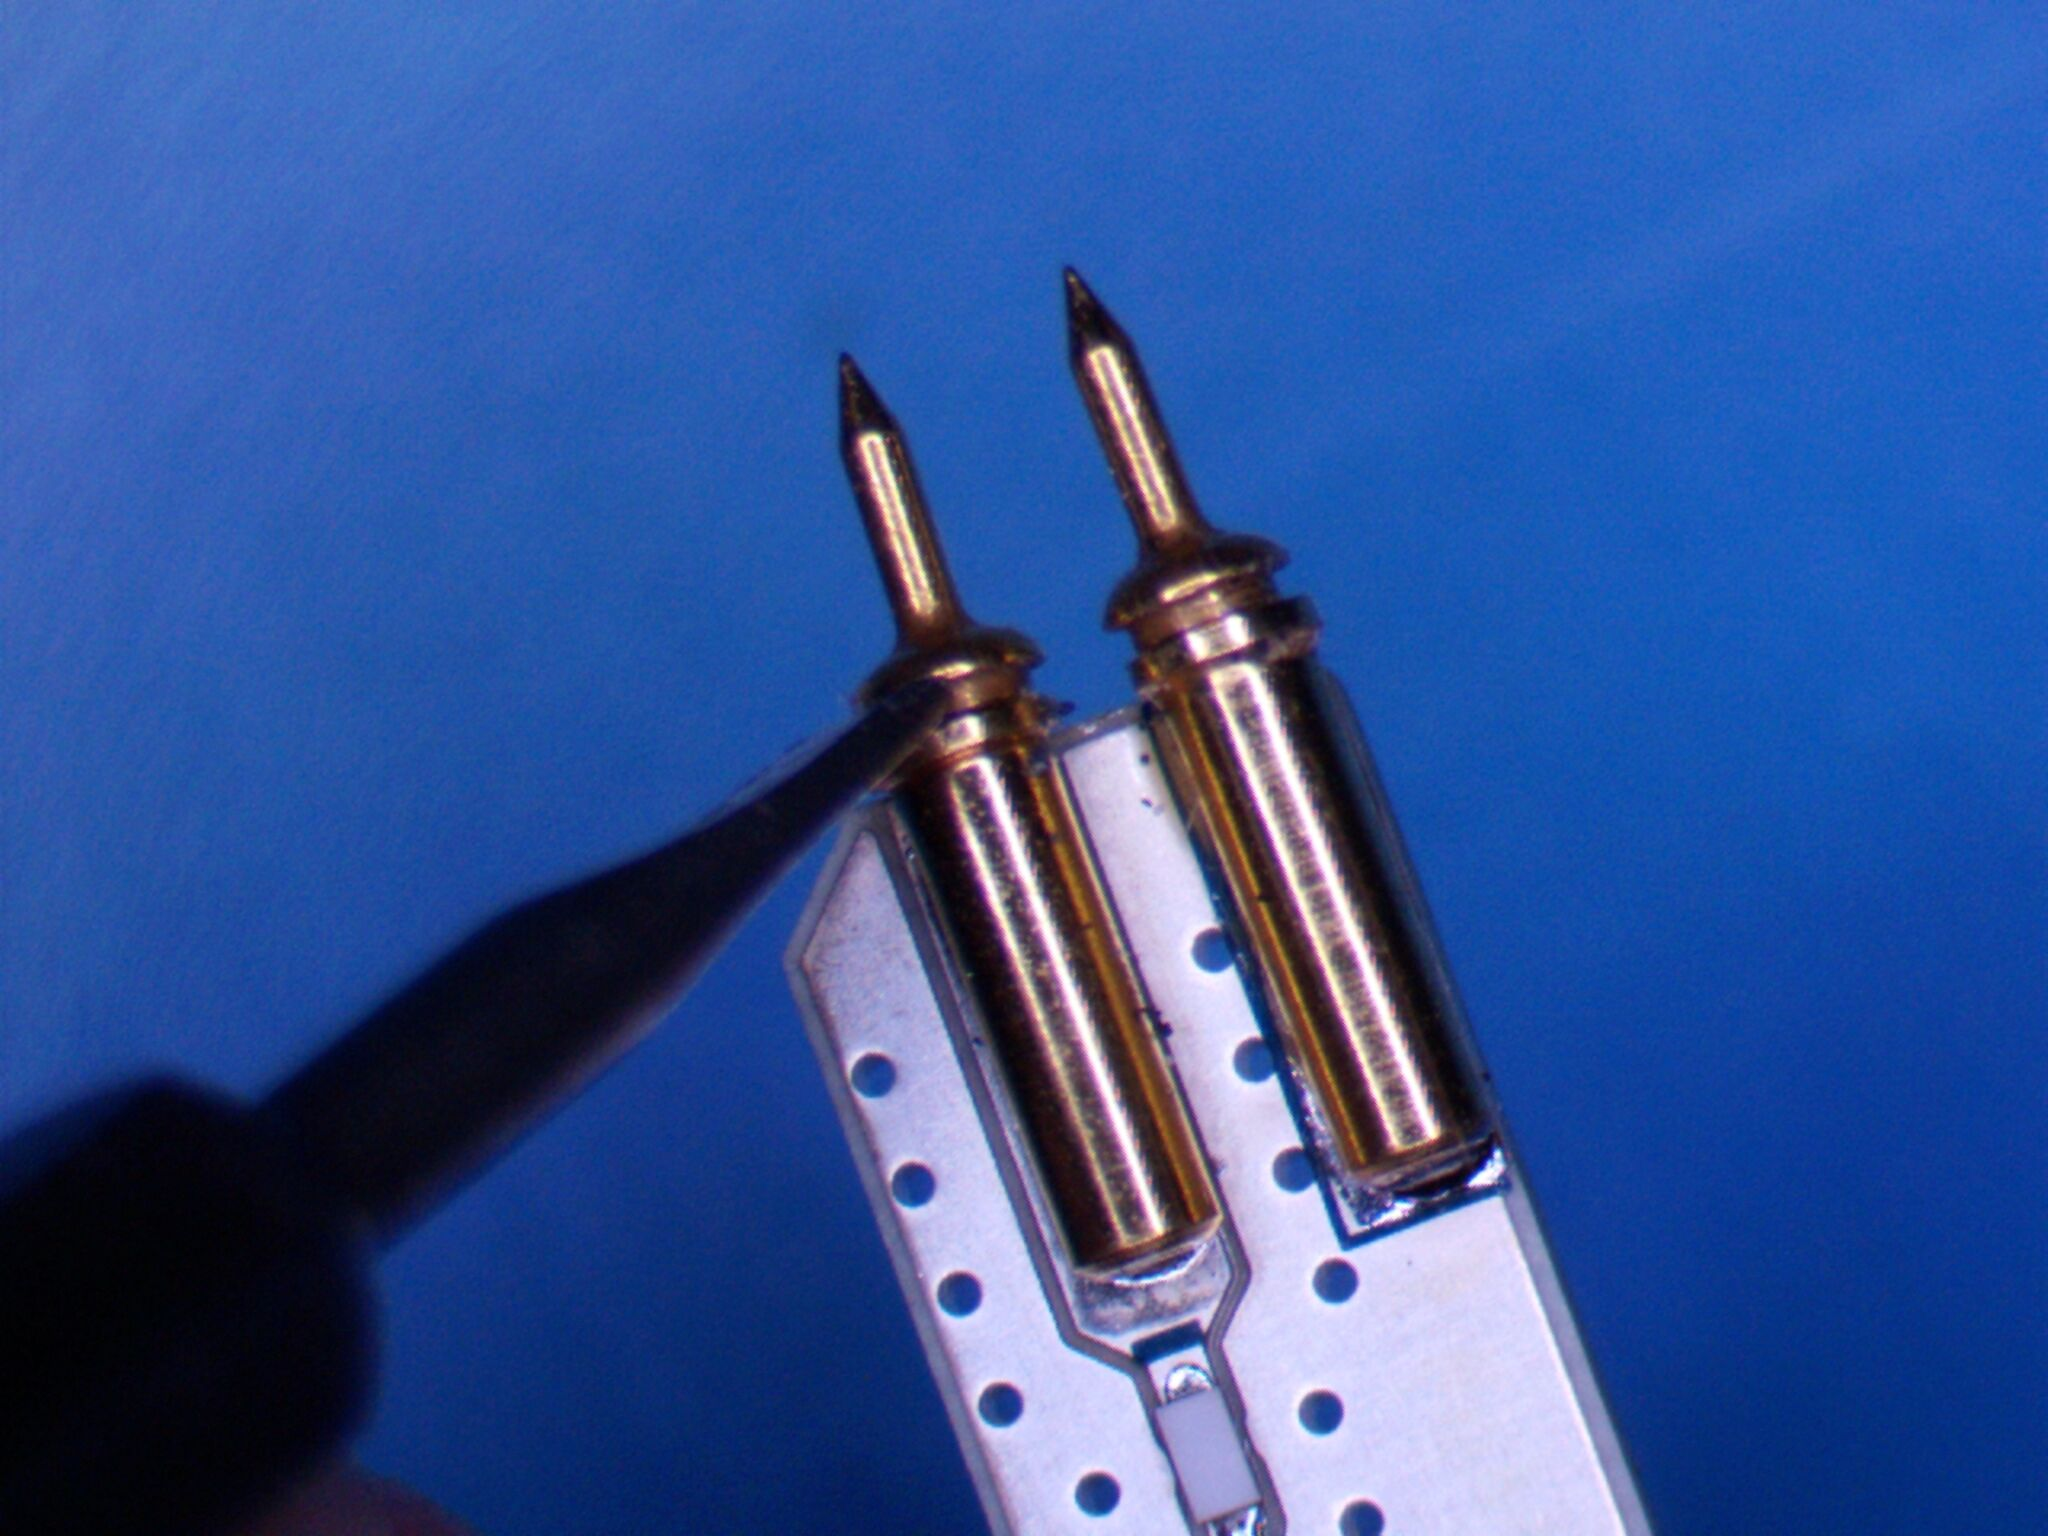
\includegraphics[width=8cm]{tip-removal.jpg}
\caption{Probe tip removal}
\end{figure}

New tips can be inserted by simply pushing them into the socket. This is best done by grasping the tip forward of the
collar, then inserting the rear of the tip into the socket and pushing until it seats fully. It is preferred to use
tweezers for this rather than holding the tip between your fingers, to avoid accidental injury.

\begin{figure}[h!]
\centering
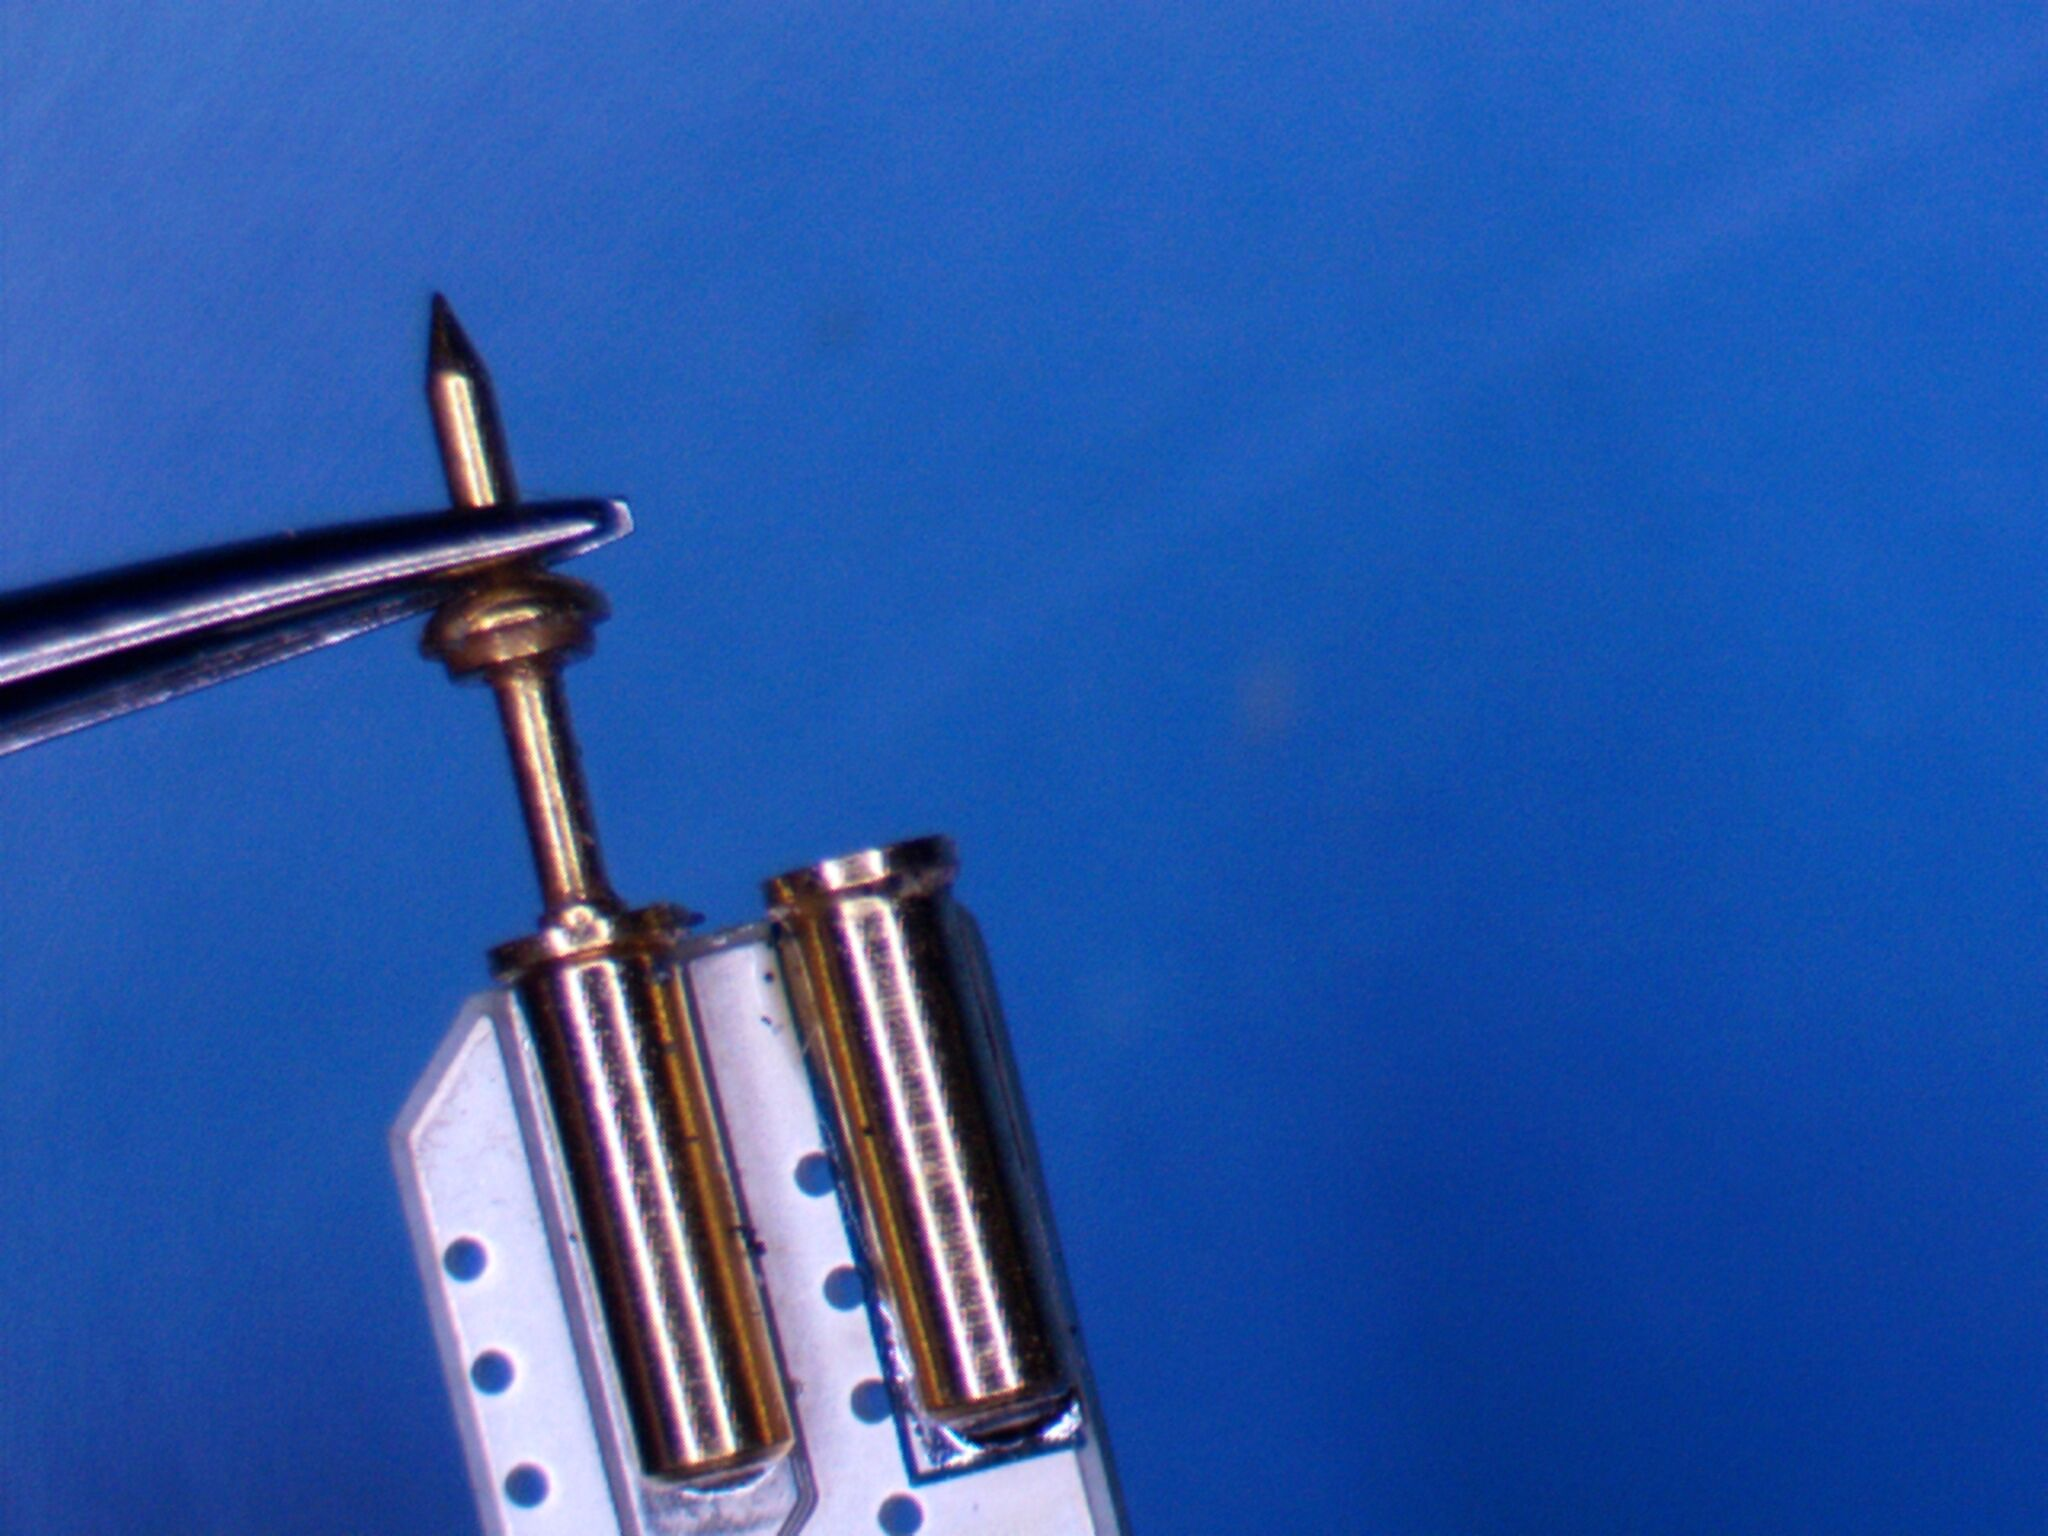
\includegraphics[width=8cm]{tip-insertion.jpg}
\caption{Inserting a tip}
\end{figure}

The probe does not require routine cleaning, however if cleaning is required for any reason it may be wiped with a damp
cloth. Isopropyl alcohol is safe to use on the plastic shell and exposed circuit board, however repeated cleaning with
alcohol may degrade the adhesive on the label. Do not use acetone or other strong solvents for cleaning.

\pagebreak
\section{Accessories}

\subsection{Tips / Grounds}

The AKL-PT1 probe sockets will accept standard test equipment probe tips and ground accessories with 0.51 - 0.81 mm
diameter (0.020 - 0.032 inch), as well as 22 AWG solid wire for solder-in applications.

Use of accessories with larger or smaller diameters may damage the socket and void your warranty.

The top ground terminal is centered 8 mm above and 12 mm to the rear of the signal connection, and the tip-mounted
ground terminal is centered 2.5mm below the signal connection.

Antikernel Labs recommends use of PMK Tetris\textsuperscript{\textregistered} series replacement probe tips and ground
accessories. These may be ordered through Antikernel Labs or any PMK distributor.

Standard PMK accessories supplied with the AKL-PT1 are:
\begin{itemize}
\item 890-800-000 solid tip (2 piece supplied standard, replacement P/N is set of 5)
\item 890-400-800 Z-ground (1 piece supplied standard, replacement P/N is set of 5)
\item 018-291-105 ground leaf
\item 890-400-808 7cm flexible ground lead
\end{itemize}

The PMK 893-250-00T 2-footed probe positioner is included with the pro edition probe.

Antikernel Labs believes the AKL-PT1 is compatible with PMK's full range of Tetris\textsuperscript{\textregistered}
tips and ground accessories, however testing has not been conducted with all possible accessories and Antikernel Labs
assumes no liability for incompatibility with any accessories not listed in this document.

\begin{figure}[h!]
\centering
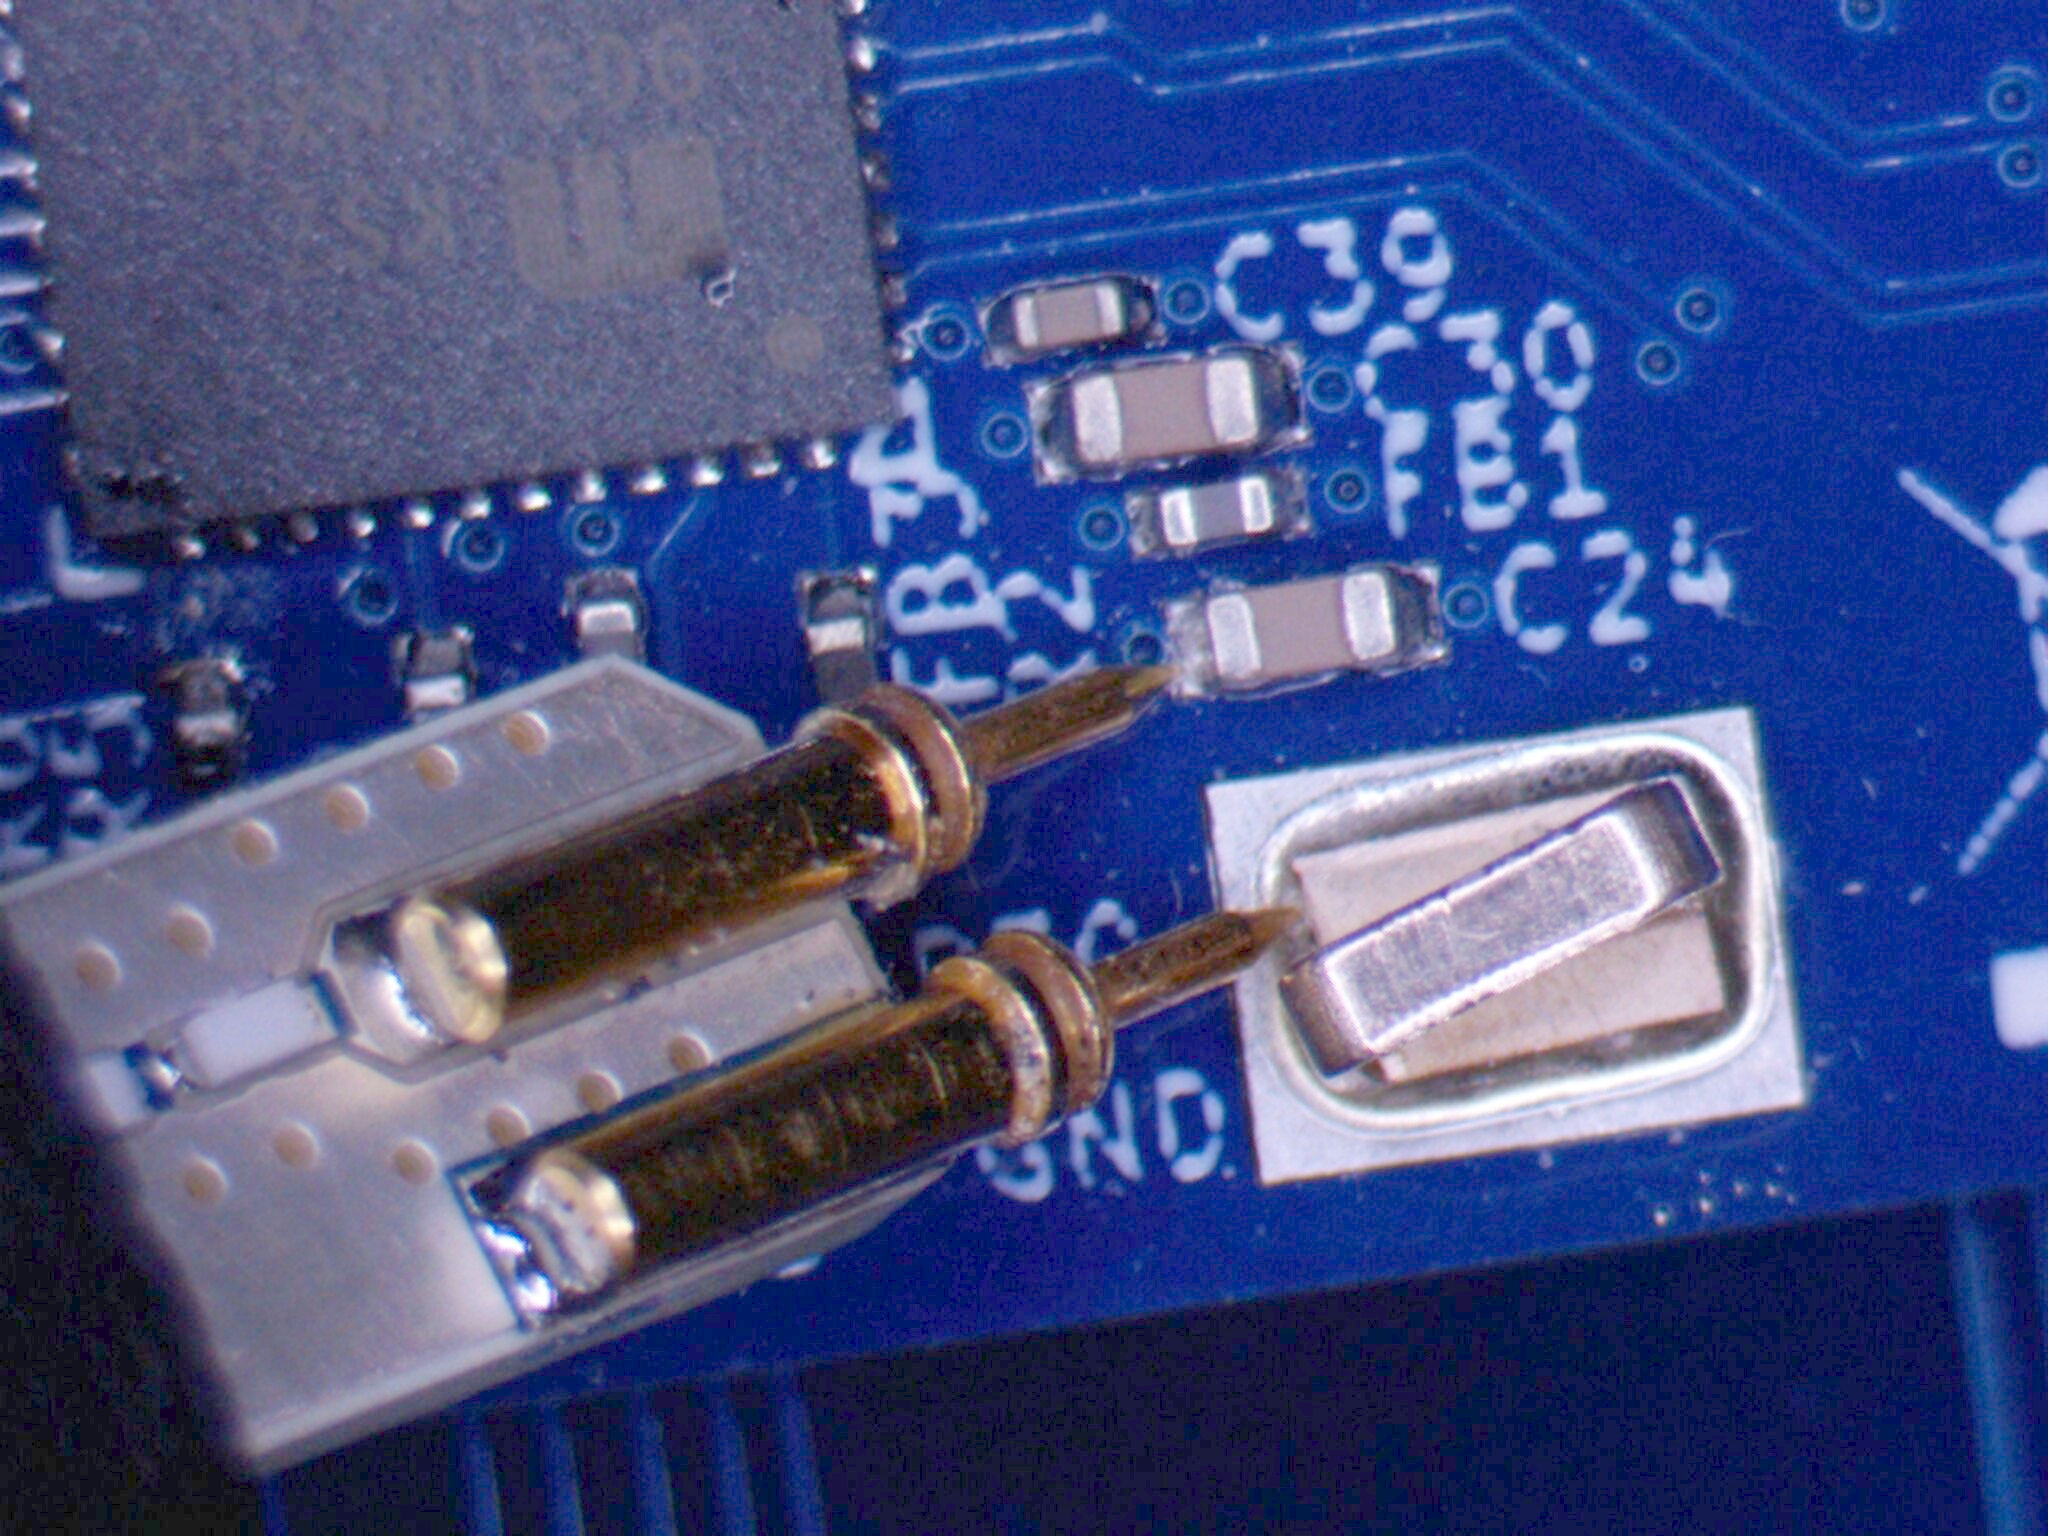
\includegraphics[width=7cm]{tip-ground-01.jpg}
\caption{Using the tip-mounted ground pin}
\end{figure}

\begin{figure}[h!]
\centering
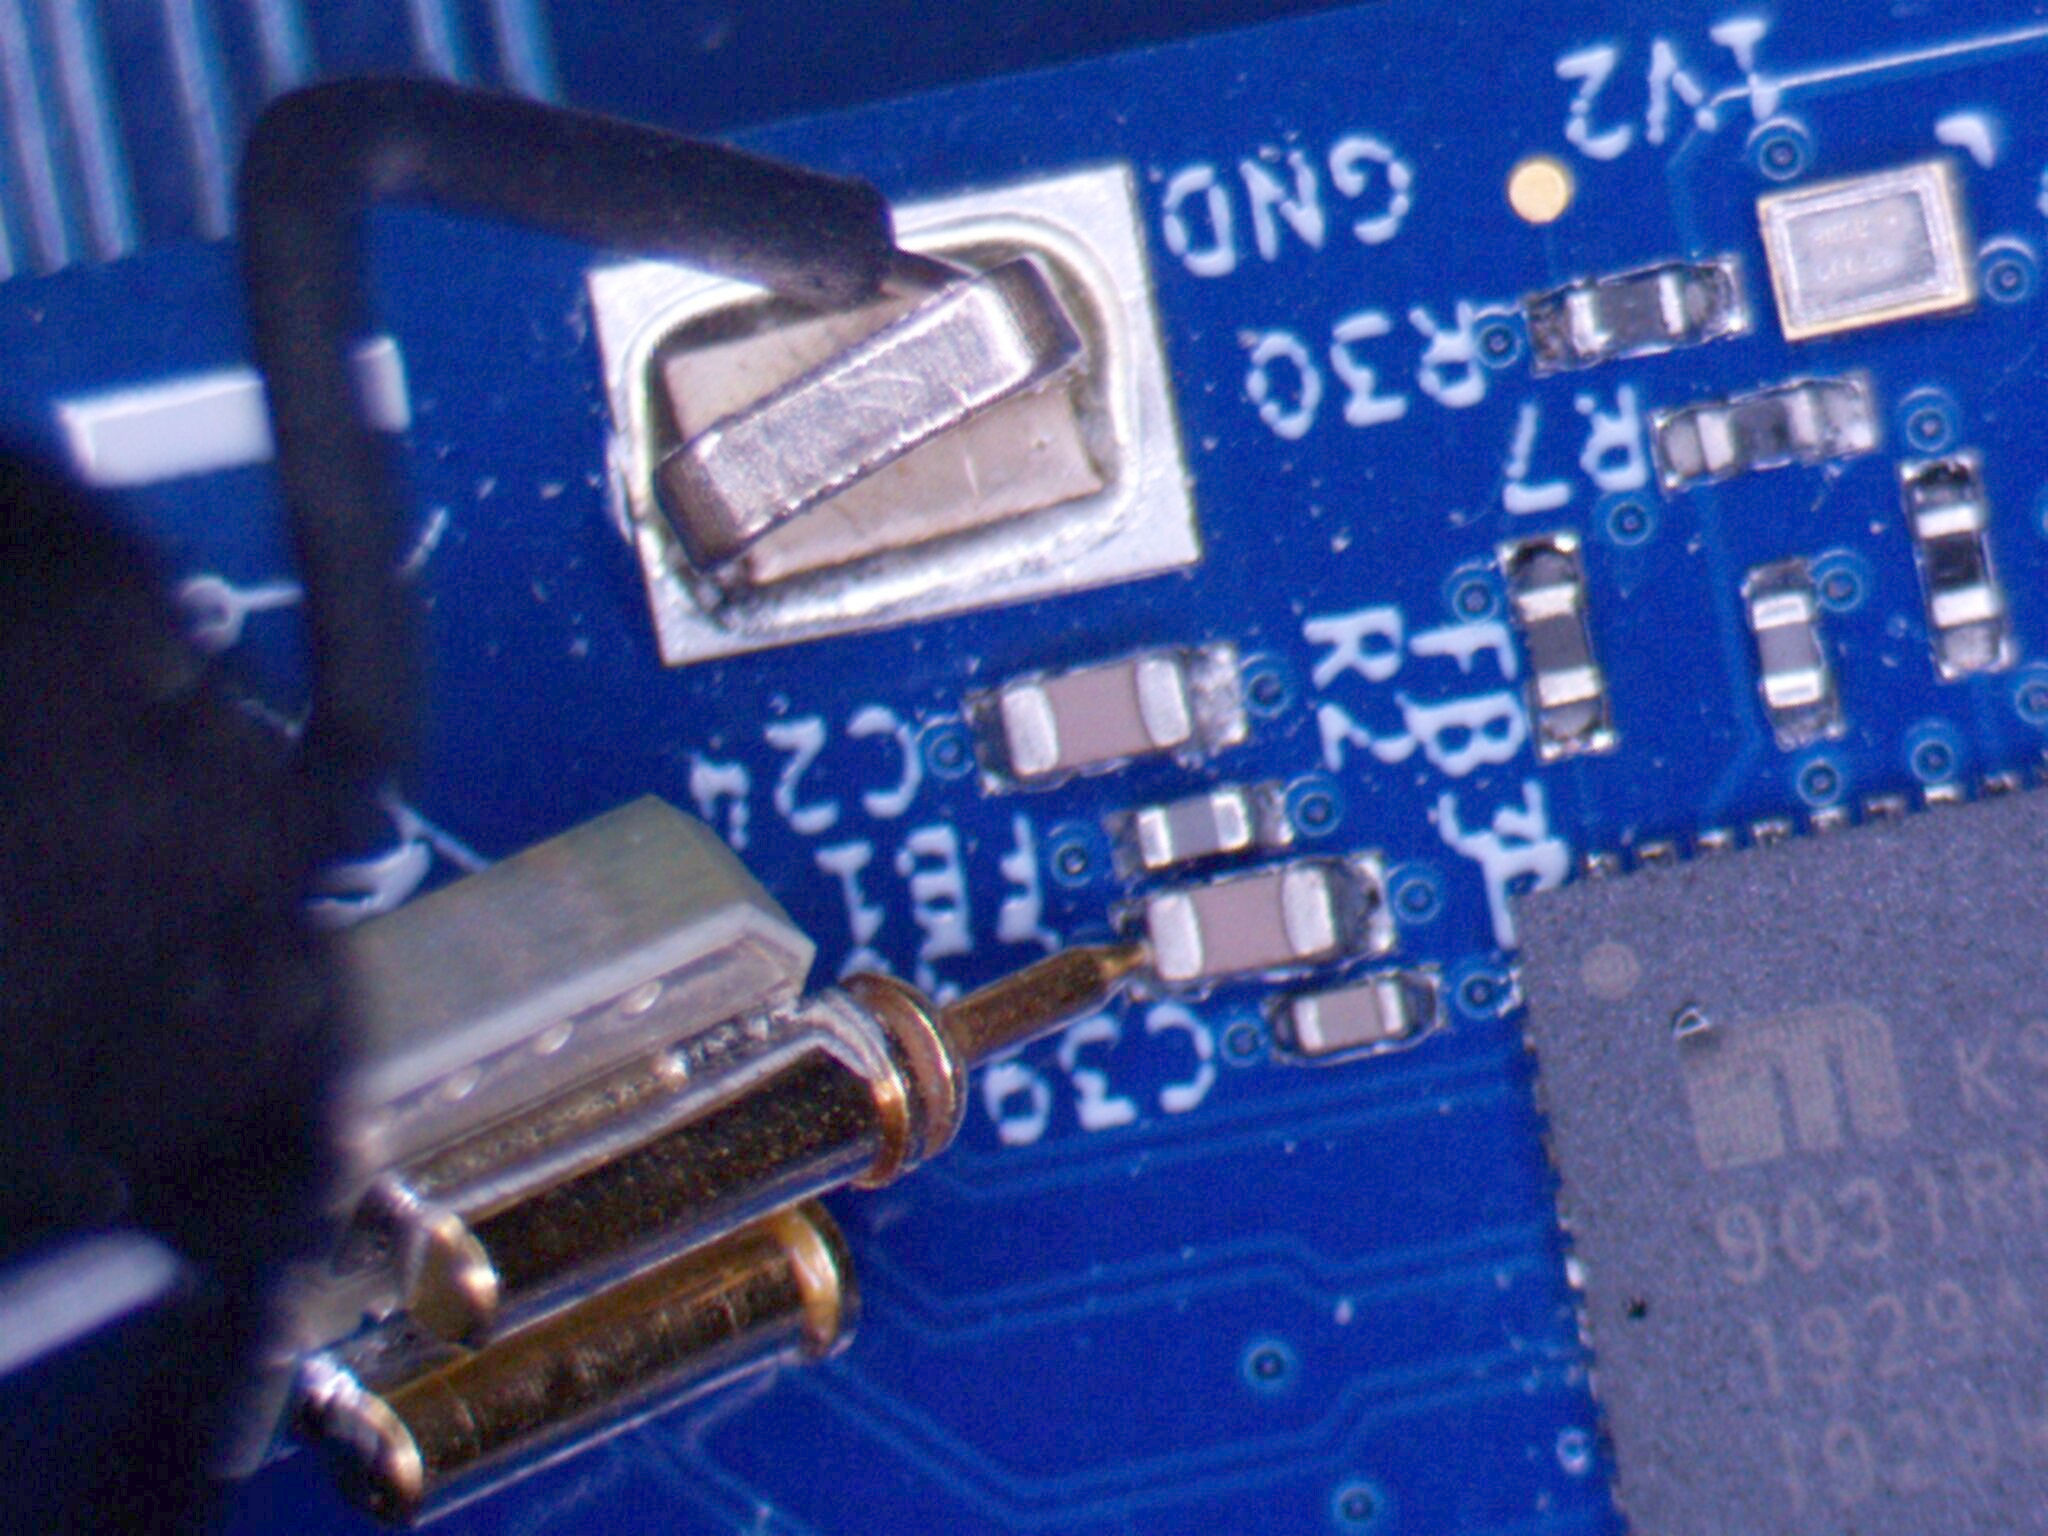
\includegraphics[width=7cm]{zground-usage.jpg}
\caption{Using the Z-ground}
\end{figure}

\begin{figure}[h!]
\centering
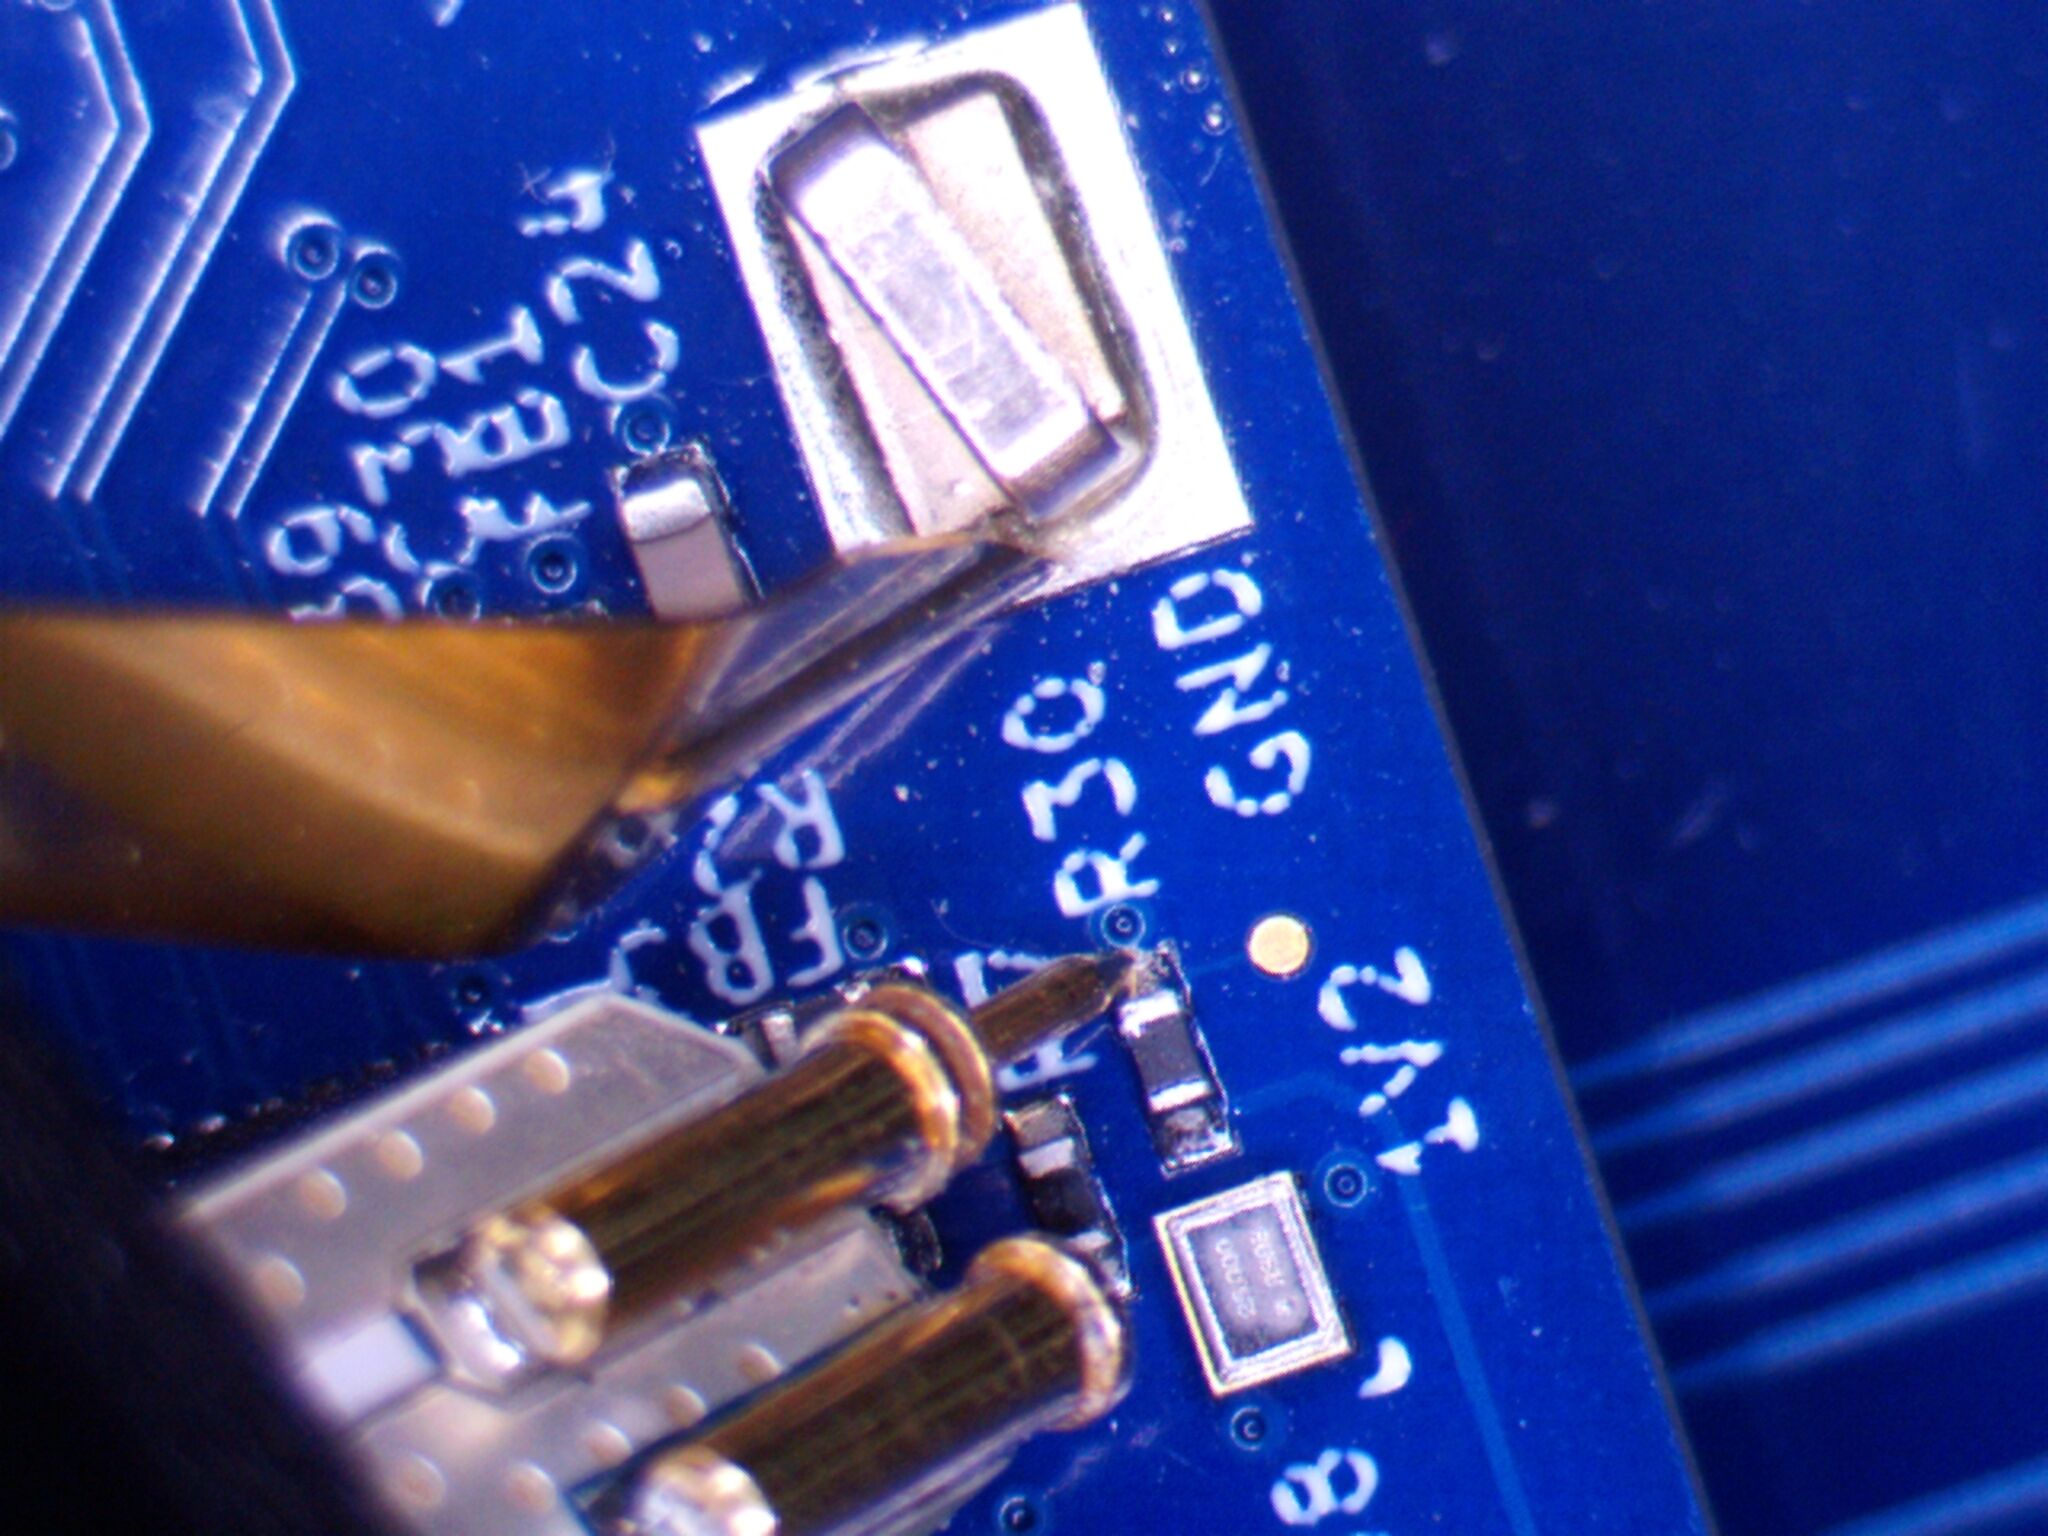
\includegraphics[width=7cm]{leafground-usage.jpg}
\caption{Using the leaf ground}
\end{figure}

\begin{figure}[h!]
\centering
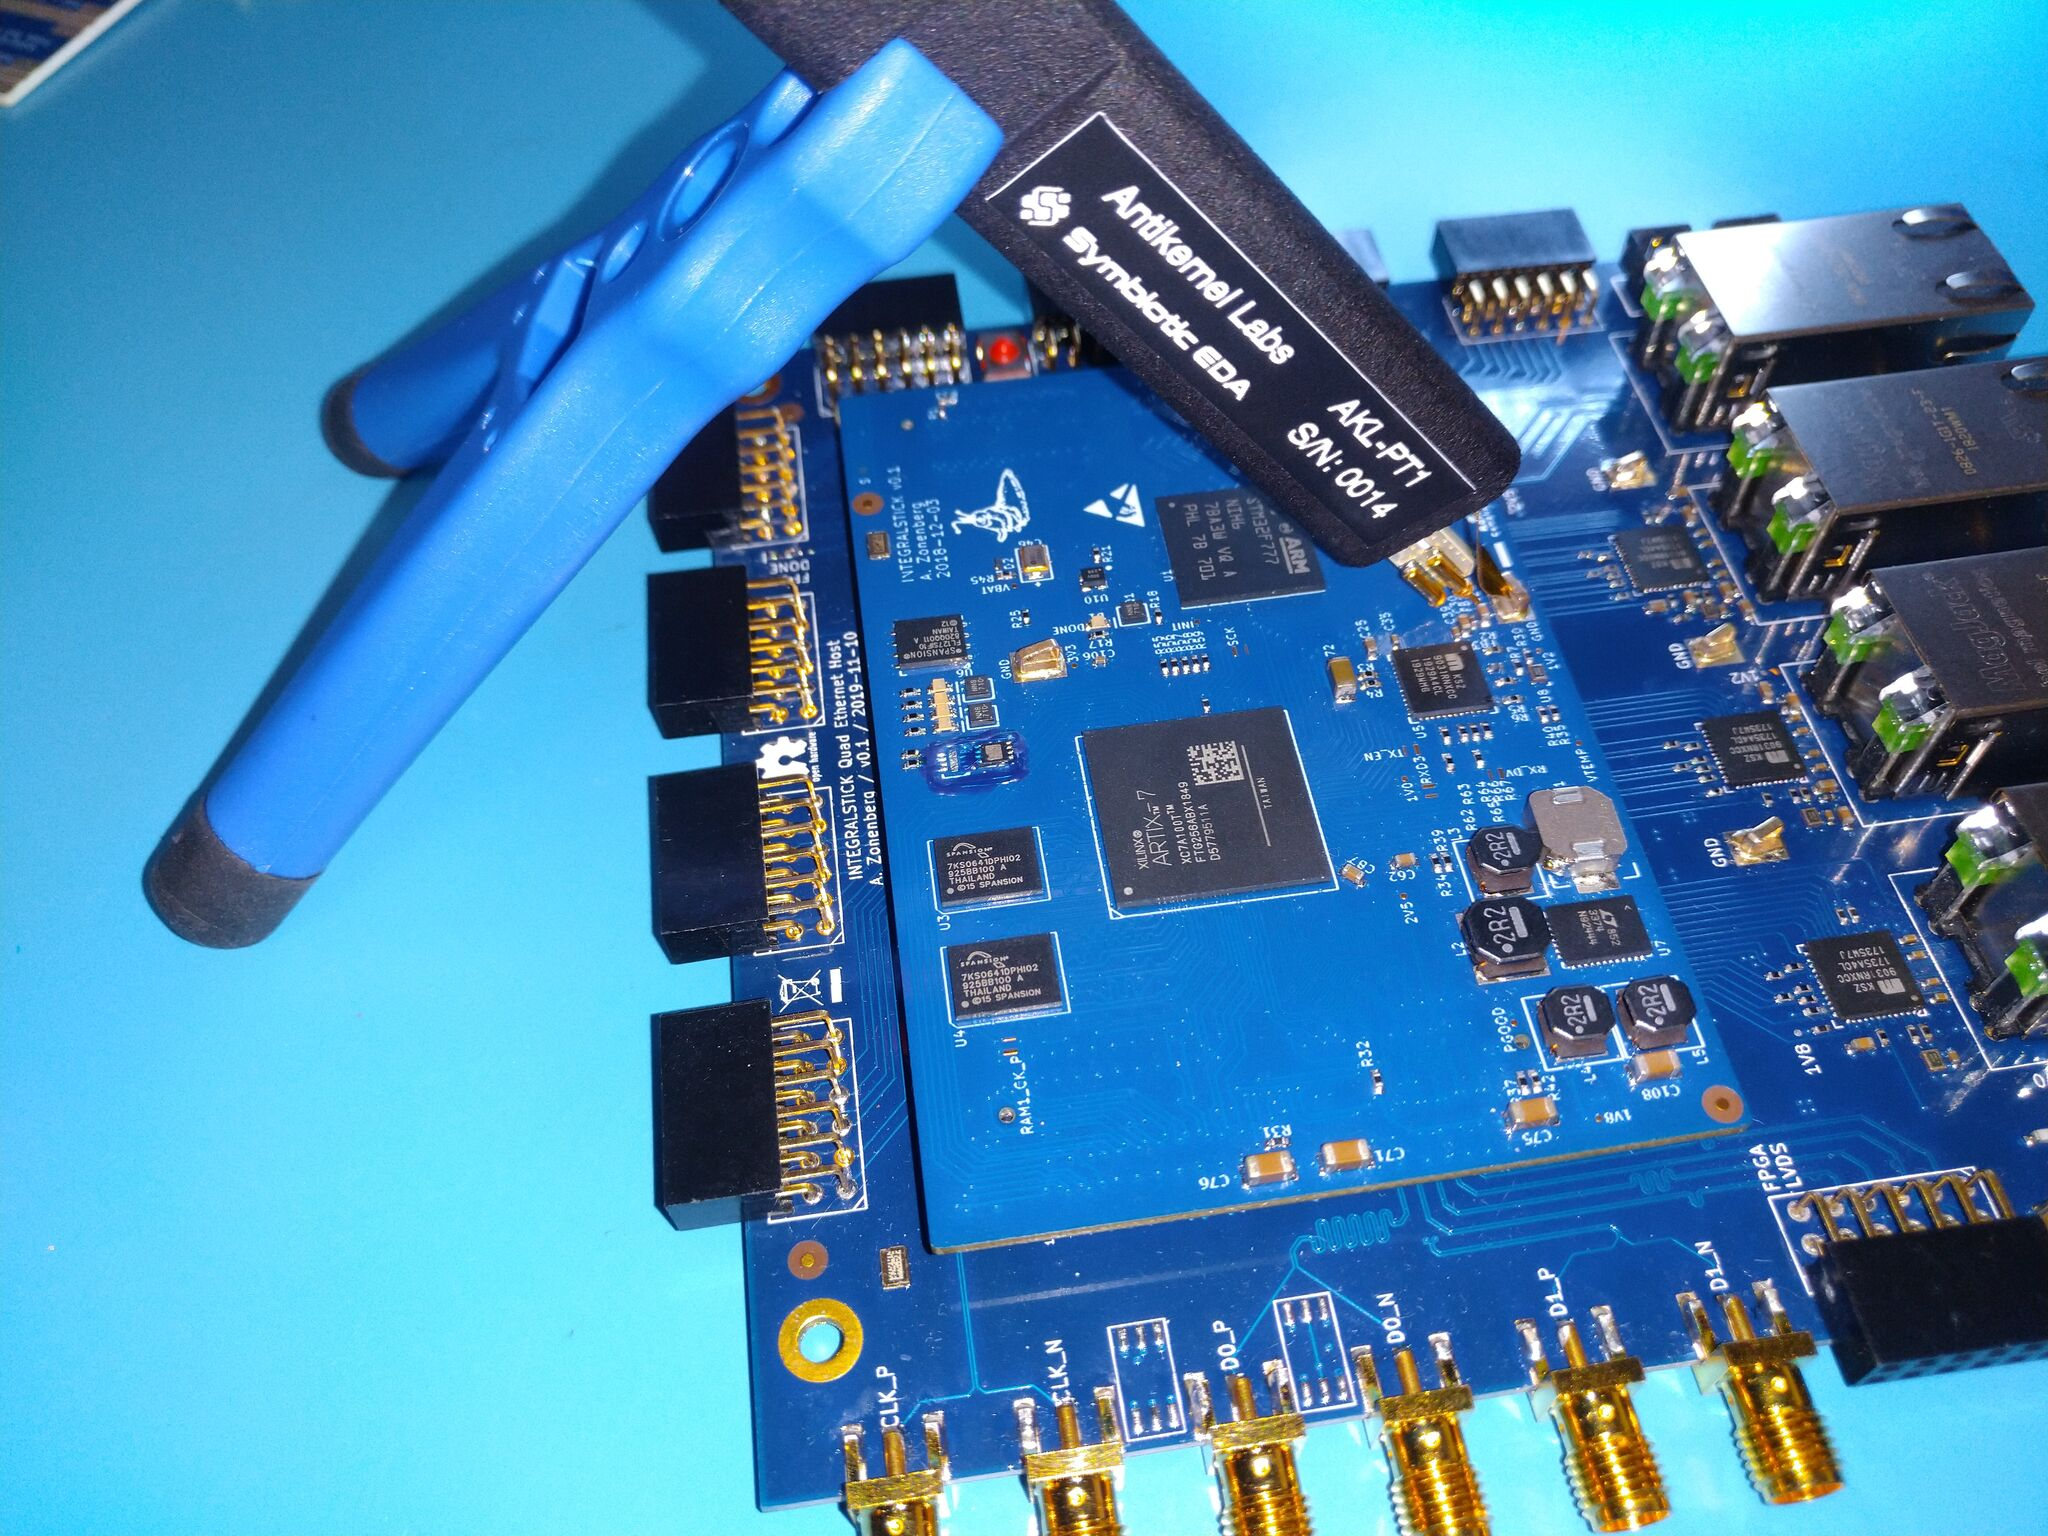
\includegraphics[width=7cm]{bipod-usage.jpg}
\caption{Using the bipod positioner}
\end{figure}

\FloatBarrier
\subsection{Cables}

The AKL-PT1 should be connected to the host instrument via a $50 \Omega$ coaxial cable (not included). Antikernel Labs
recommends use of Mini-Circuits FL086-24SM+ or similar low-loss, flexible cabling.

The probe-side connector is a brass SMA (Samtec SMA-J-P-H-ST-EM1). For best results, this connection should be torqued
to 5 in-lbf (0.57 Nm). Over-tightening may damage the connector.

\pagebreak
\section{Electrical Specifications}

Values in this section are typical / limit values. For measured values from a specific probe, please consult your
calibration certificate.

% Assume 0.0015x worst case for resistor base tolerance
% 25 ppm (0.000025x) per degC, -10 / +20C range gives -0.00025 / +0.0005x
% so final range is 0.9975 / 1.005

\subsection{Absolute Maximum Ratings}

Exceeding these limits may result in permanent damage to the probe.

Ratings in this section are stress ratings only and normal operation at these limits is not implied.

\begin{tabularx}{16cm}{lXll}
\thickhline
\textbf{Parameter} & \textbf{Description} & \textbf{Limit} & \textbf{Units} \\
\thickhline
$T_{amin}$ & Minimum temperature & 0 & $ \degree C$ \\
\thinhline
$T_{amax}$ & Maximum temperature & 95 & $ \degree C$ \\
\thinhline
$I_{max}$ & Maximum current through probe & 22 & $ mA $ \\
\thinhline
$V_{max}$ & Maximum operating voltage & 10 & $ Vrms $ \\
\thickhline
\end{tabularx}

\subsection{Recommended Operating Conditions}

While the probe will not be damaged by exposure to conditions outside the values in this section (but below the
``Absolute Maximum Ratings" limits), tolerances may be temporarily exceeded.

\begin{tabularx}{16cm}{lXll}
\thickhline
\textbf{Parameter} & \textbf{Description} & \textbf{Limit} & \textbf{Units} \\
\thickhline
$T_{min}$ & Minimum temperature & 15 & \degree C \\
\thinhline
$T_{max}$ & Maximum temperature & 45 & \degree C \\
\thinhline
\thickhline
\end{tabularx}

\subsection{DC Characteristics}

\begin{tabularx}{16cm}{lXrrrr}
\thickhline
\textbf{Parameter} & \textbf{Description} & \textbf{Min} & \textbf{Typ} & \textbf{Max} & \textbf{Units} \\
\thickhline
$G_{dc}$ & DC gain & 0.0997 & 0.1000 & 0.1005 & V/V \\
\thinhline
$R_{25}$ & DC resistance of probe (25 \degree C) & 449.75 & 450.31 & 450.75 & $\Omega$ \\
\thinhline
$R_{range}$ & DC resistance of probe (15 - 45 \degree C) & 449.60 & 450.31 & 451.00 & $\Omega$ \\
\thinhline
$TCR$ & Temperature coefficient of resistance & & & $\pm 25$ & ppm / \degree C \\
\thickhline
\end{tabularx}

\pagebreak
\subsection{AC Characteristics}

Data in this section is based on characterization in a $50 \Omega$ environment, using the highest performance (tip)
ground, with cable and fixture effects de-embedded, unless otherwise stated.

\begin{tabularx}{16cm}{lXrrrr}
\thickhline
\textbf{Parameter} & \textbf{Description} & \textbf{Min} & \textbf{Typ} & \textbf{Max} & \textbf{Units} \\
\thickhline
$Z_{in1}$ & Input impedance (1 GHz) & 82.00 & 86.05 & 88.00 & $\Omega$ \\
\thinhline
$Z_{in2}$ & Input impedance (2 GHz) & 29.00 & 30.79 & 32.75 & $\Omega$ \\
\thinhline
$C_{in}$ & Equivalent shunt capacitance to ground &  & 1.4 &  & pF \\
\thinhline
$G$ & AC gain from DC - 2 GHz & -23 & -20.5 & -20 & dB \\
\thinhline
$G_1$ & AC gain at 1 MHz & -20.48 & -20.45 & -20.42 & dB \\
\thinhline
$G_{500}$ & AC gain at 0.5 GHz & -20.85 & -20.56 & -20.35 & dB \\
\thinhline
$G_{1000}$ & AC gain at 1.0 GHz & -21.10 & -20.81 & -20.35 & dB \\
\thinhline
$G_{1500}$ & AC gain at 1.5 GHz & -21.45 & -21.17 & -20.75 & dB \\
\thinhline
$G_{2000}$ & AC gain at 2.0 GHz & -21.60 & -22.04 & -22.45 & dB \\
\thinhline
$BW_{0.5}$ & $\pm 0.5$ dB bandwidth using tip ground &  & 0.91 & & GHz \\
\thinhline
$BW_{3}$ & -3 dB bandwidth using tip ground & 2.25 & 2.47 & 2.60 & GHz \\
\thinhline
$BW_{flex}$ & -3 dB bandwidth using flex ground &  & 0.56 &  & GHz \\
\thinhline
$BW_{leaf}$ & -3 dB bandwidth using leaf ground &  & 1.46 &  & GHz \\
\thinhline
$BW_{z}$ & -3 dB bandwidth using Z-ground &  & 0.80 &  & GHz \\
\thinhline
$Rise_{90}$ & Rise time (10-90 \%, including cable) & 174 & 179 & 189 & ps \\
\thinhline
$Rise_{80}$ & Rise time (20-80 \%, including cable) & 118 & 122 & 129 & ps \\
\thinhline
$Tpd$ & Propagation delay &  & 548 &  & ps \\
\thickhline
\end{tabularx}

\pagebreak
\section{Performance Graphs}

\subsection{Insertion Loss}

Measured across a $50 \Omega$ termination.

\begin{figure}[h]
\centering
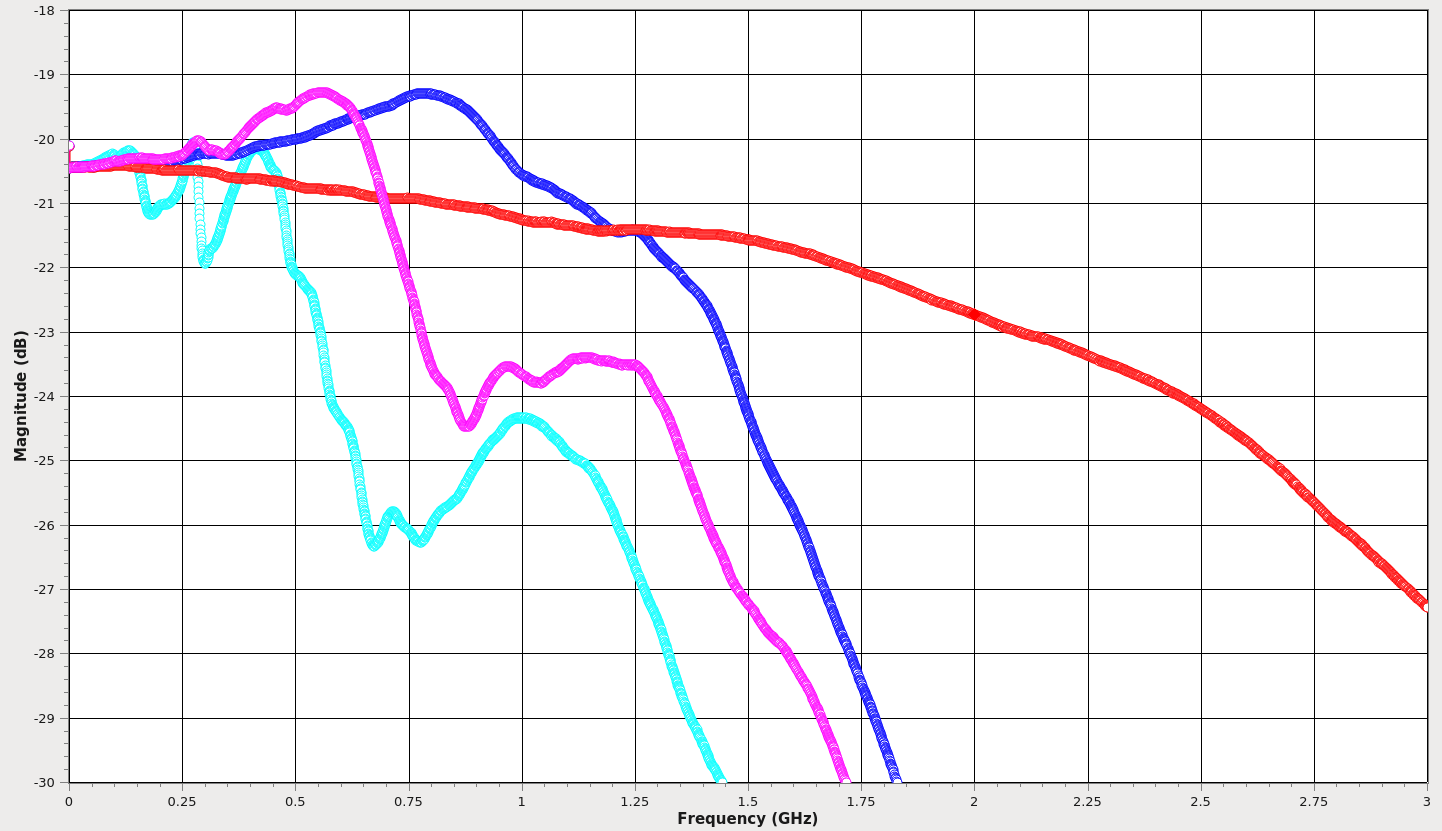
\includegraphics[width=14cm]{typical-s21.png}
\caption{Typical $S_{21}$ using tip ground (red), leaf ground (blue), Z-ground (pink), flex ground (cyan)}
\end{figure}

\begin{figure}[h]
\centering
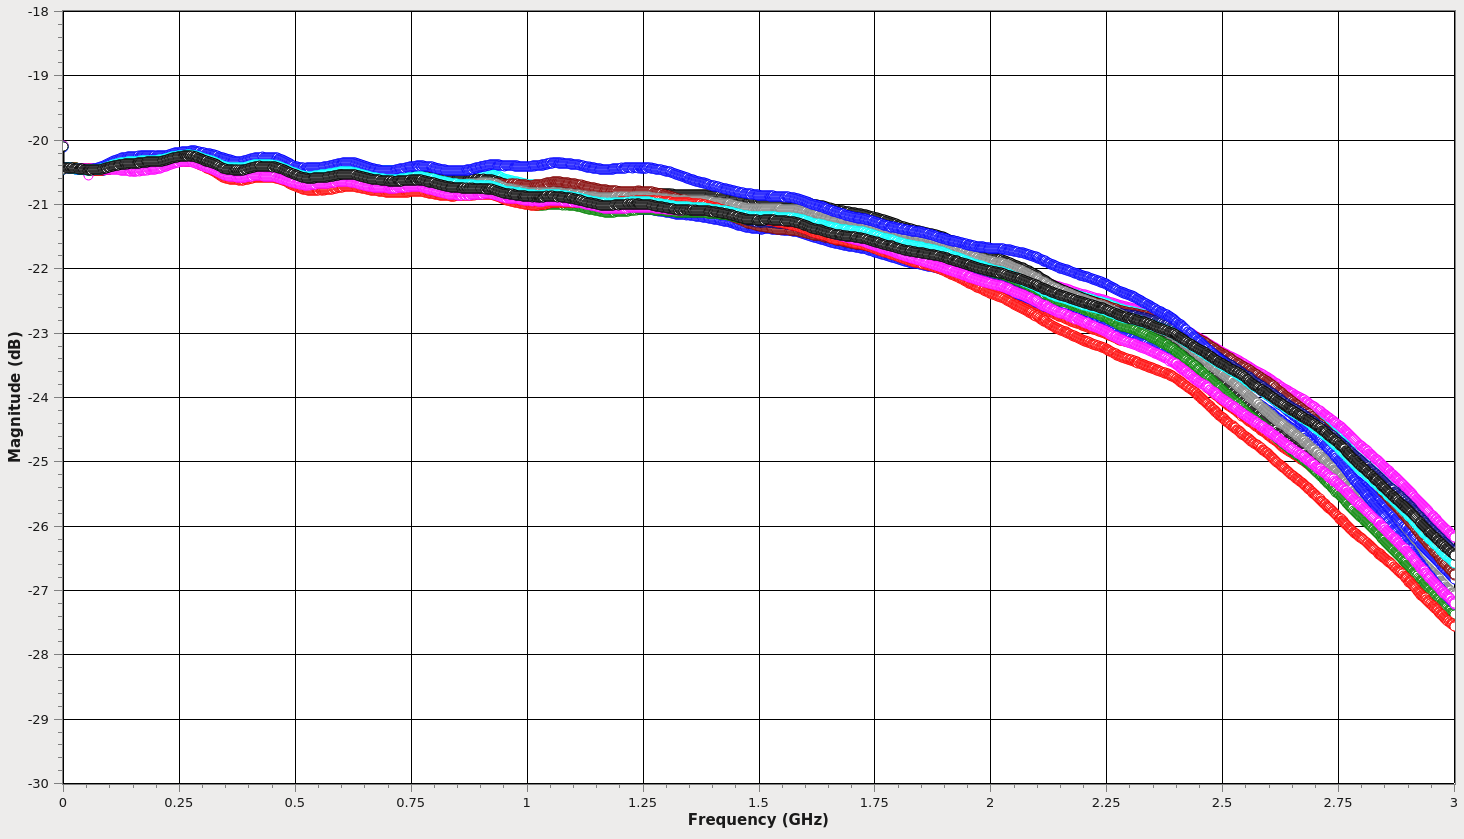
\includegraphics[width=14cm]{s21-spread.png}
\caption{Unit to unit variation in $S_{21}$}
\end{figure}

\pagebreak
\subsection{Group Delay}

\begin{figure}[h]
\centering
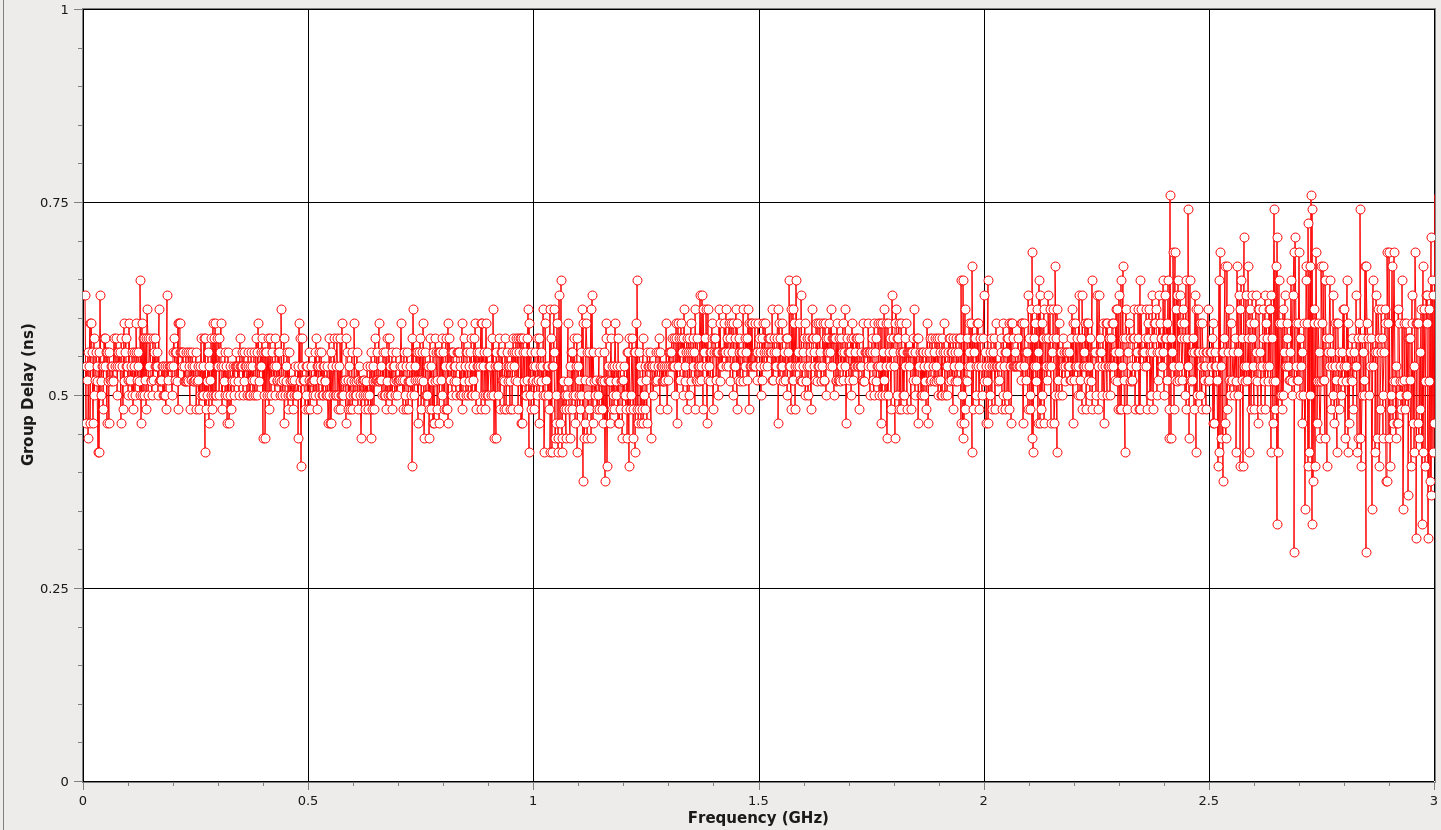
\includegraphics[width=14cm]{typical-groupdelay.png}
\caption{Typical Group Delay Flatness}
\label{typical-groupdelay}
\end{figure}
\FloatBarrier

\subsection{Input Impedance}

\begin{figure}[h!]
\centering
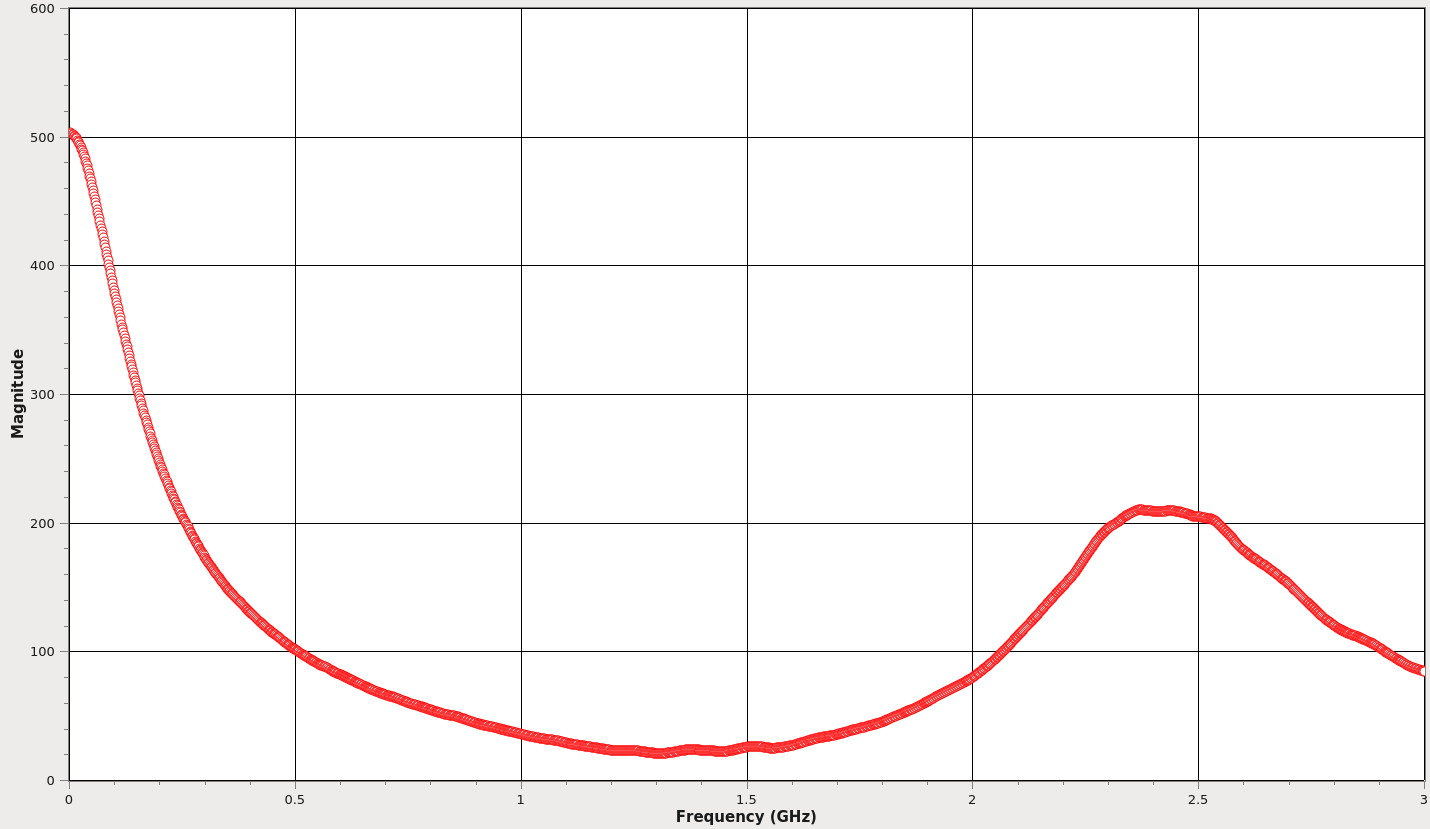
\includegraphics[width=14cm]{typical-zin.png}
\caption{Typical $Z_{in}$}
\label{typical-zin}
\end{figure}

\FloatBarrier

\pagebreak
\section{Performance Data}

If you requested full characterization at the time of your order, test measurements are available at
\url{https://www.github.com/azonenberg/starshipraider-caldata/tree/master/handheld-resistive-probe/} under the
directory for your probe's serial number.

The following S-parameter data files are provided:
\begin{itemize}
\item cable.s2p - the provided cable
\item flexground.s2p - probe across a $50 \Omega$ load using the flex ground
\item leafground.s2p - probe across a $50 \Omega$ load using the leaf ground
\item tipground.s2p - probe across a $50 \Omega$ load using the tip ground
\item zground.s2p - probe across a $50 \Omega$ load using the Z-ground
\item zin.s2p - probe across an unterminated line for input loading measurements
\end{itemize}

For all measurements, port 1 is connected to the DUT side of the probe and port 2 is connected to the instrument side.

\end{document}
